% Options for packages loaded elsewhere
\PassOptionsToPackage{unicode}{hyperref}
\PassOptionsToPackage{hyphens}{url}
\PassOptionsToPackage{dvipsnames,svgnames,x11names}{xcolor}
%
\documentclass[
  letterpaper,
  DIV=11,
  numbers=noendperiod]{scrartcl}

\usepackage{amsmath,amssymb}
\usepackage{iftex}
\ifPDFTeX
  \usepackage[T1]{fontenc}
  \usepackage[utf8]{inputenc}
  \usepackage{textcomp} % provide euro and other symbols
\else % if luatex or xetex
  \usepackage{unicode-math}
  \defaultfontfeatures{Scale=MatchLowercase}
  \defaultfontfeatures[\rmfamily]{Ligatures=TeX,Scale=1}
\fi
\usepackage{lmodern}
\ifPDFTeX\else  
    % xetex/luatex font selection
\fi
% Use upquote if available, for straight quotes in verbatim environments
\IfFileExists{upquote.sty}{\usepackage{upquote}}{}
\IfFileExists{microtype.sty}{% use microtype if available
  \usepackage[]{microtype}
  \UseMicrotypeSet[protrusion]{basicmath} % disable protrusion for tt fonts
}{}
\makeatletter
\@ifundefined{KOMAClassName}{% if non-KOMA class
  \IfFileExists{parskip.sty}{%
    \usepackage{parskip}
  }{% else
    \setlength{\parindent}{0pt}
    \setlength{\parskip}{6pt plus 2pt minus 1pt}}
}{% if KOMA class
  \KOMAoptions{parskip=half}}
\makeatother
\usepackage{xcolor}
\setlength{\emergencystretch}{3em} % prevent overfull lines
\setcounter{secnumdepth}{5}
% Make \paragraph and \subparagraph free-standing
\ifx\paragraph\undefined\else
  \let\oldparagraph\paragraph
  \renewcommand{\paragraph}[1]{\oldparagraph{#1}\mbox{}}
\fi
\ifx\subparagraph\undefined\else
  \let\oldsubparagraph\subparagraph
  \renewcommand{\subparagraph}[1]{\oldsubparagraph{#1}\mbox{}}
\fi

\usepackage{color}
\usepackage{fancyvrb}
\newcommand{\VerbBar}{|}
\newcommand{\VERB}{\Verb[commandchars=\\\{\}]}
\DefineVerbatimEnvironment{Highlighting}{Verbatim}{commandchars=\\\{\}}
% Add ',fontsize=\small' for more characters per line
\usepackage{framed}
\definecolor{shadecolor}{RGB}{241,243,245}
\newenvironment{Shaded}{\begin{snugshade}}{\end{snugshade}}
\newcommand{\AlertTok}[1]{\textcolor[rgb]{0.68,0.00,0.00}{#1}}
\newcommand{\AnnotationTok}[1]{\textcolor[rgb]{0.37,0.37,0.37}{#1}}
\newcommand{\AttributeTok}[1]{\textcolor[rgb]{0.40,0.45,0.13}{#1}}
\newcommand{\BaseNTok}[1]{\textcolor[rgb]{0.68,0.00,0.00}{#1}}
\newcommand{\BuiltInTok}[1]{\textcolor[rgb]{0.00,0.23,0.31}{#1}}
\newcommand{\CharTok}[1]{\textcolor[rgb]{0.13,0.47,0.30}{#1}}
\newcommand{\CommentTok}[1]{\textcolor[rgb]{0.37,0.37,0.37}{#1}}
\newcommand{\CommentVarTok}[1]{\textcolor[rgb]{0.37,0.37,0.37}{\textit{#1}}}
\newcommand{\ConstantTok}[1]{\textcolor[rgb]{0.56,0.35,0.01}{#1}}
\newcommand{\ControlFlowTok}[1]{\textcolor[rgb]{0.00,0.23,0.31}{#1}}
\newcommand{\DataTypeTok}[1]{\textcolor[rgb]{0.68,0.00,0.00}{#1}}
\newcommand{\DecValTok}[1]{\textcolor[rgb]{0.68,0.00,0.00}{#1}}
\newcommand{\DocumentationTok}[1]{\textcolor[rgb]{0.37,0.37,0.37}{\textit{#1}}}
\newcommand{\ErrorTok}[1]{\textcolor[rgb]{0.68,0.00,0.00}{#1}}
\newcommand{\ExtensionTok}[1]{\textcolor[rgb]{0.00,0.23,0.31}{#1}}
\newcommand{\FloatTok}[1]{\textcolor[rgb]{0.68,0.00,0.00}{#1}}
\newcommand{\FunctionTok}[1]{\textcolor[rgb]{0.28,0.35,0.67}{#1}}
\newcommand{\ImportTok}[1]{\textcolor[rgb]{0.00,0.46,0.62}{#1}}
\newcommand{\InformationTok}[1]{\textcolor[rgb]{0.37,0.37,0.37}{#1}}
\newcommand{\KeywordTok}[1]{\textcolor[rgb]{0.00,0.23,0.31}{#1}}
\newcommand{\NormalTok}[1]{\textcolor[rgb]{0.00,0.23,0.31}{#1}}
\newcommand{\OperatorTok}[1]{\textcolor[rgb]{0.37,0.37,0.37}{#1}}
\newcommand{\OtherTok}[1]{\textcolor[rgb]{0.00,0.23,0.31}{#1}}
\newcommand{\PreprocessorTok}[1]{\textcolor[rgb]{0.68,0.00,0.00}{#1}}
\newcommand{\RegionMarkerTok}[1]{\textcolor[rgb]{0.00,0.23,0.31}{#1}}
\newcommand{\SpecialCharTok}[1]{\textcolor[rgb]{0.37,0.37,0.37}{#1}}
\newcommand{\SpecialStringTok}[1]{\textcolor[rgb]{0.13,0.47,0.30}{#1}}
\newcommand{\StringTok}[1]{\textcolor[rgb]{0.13,0.47,0.30}{#1}}
\newcommand{\VariableTok}[1]{\textcolor[rgb]{0.07,0.07,0.07}{#1}}
\newcommand{\VerbatimStringTok}[1]{\textcolor[rgb]{0.13,0.47,0.30}{#1}}
\newcommand{\WarningTok}[1]{\textcolor[rgb]{0.37,0.37,0.37}{\textit{#1}}}

\providecommand{\tightlist}{%
  \setlength{\itemsep}{0pt}\setlength{\parskip}{0pt}}\usepackage{longtable,booktabs,array}
\usepackage{calc} % for calculating minipage widths
% Correct order of tables after \paragraph or \subparagraph
\usepackage{etoolbox}
\makeatletter
\patchcmd\longtable{\par}{\if@noskipsec\mbox{}\fi\par}{}{}
\makeatother
% Allow footnotes in longtable head/foot
\IfFileExists{footnotehyper.sty}{\usepackage{footnotehyper}}{\usepackage{footnote}}
\makesavenoteenv{longtable}
\usepackage{graphicx}
\makeatletter
\def\maxwidth{\ifdim\Gin@nat@width>\linewidth\linewidth\else\Gin@nat@width\fi}
\def\maxheight{\ifdim\Gin@nat@height>\textheight\textheight\else\Gin@nat@height\fi}
\makeatother
% Scale images if necessary, so that they will not overflow the page
% margins by default, and it is still possible to overwrite the defaults
% using explicit options in \includegraphics[width, height, ...]{}
\setkeys{Gin}{width=\maxwidth,height=\maxheight,keepaspectratio}
% Set default figure placement to htbp
\makeatletter
\def\fps@figure{htbp}
\makeatother

\KOMAoption{captions}{tableheading}
\makeatletter
\makeatother
\makeatletter
\makeatother
\makeatletter
\@ifpackageloaded{caption}{}{\usepackage{caption}}
\AtBeginDocument{%
\ifdefined\contentsname
  \renewcommand*\contentsname{Table of contents}
\else
  \newcommand\contentsname{Table of contents}
\fi
\ifdefined\listfigurename
  \renewcommand*\listfigurename{List of Figures}
\else
  \newcommand\listfigurename{List of Figures}
\fi
\ifdefined\listtablename
  \renewcommand*\listtablename{List of Tables}
\else
  \newcommand\listtablename{List of Tables}
\fi
\ifdefined\figurename
  \renewcommand*\figurename{Figure}
\else
  \newcommand\figurename{Figure}
\fi
\ifdefined\tablename
  \renewcommand*\tablename{Table}
\else
  \newcommand\tablename{Table}
\fi
}
\@ifpackageloaded{float}{}{\usepackage{float}}
\floatstyle{ruled}
\@ifundefined{c@chapter}{\newfloat{codelisting}{h}{lop}}{\newfloat{codelisting}{h}{lop}[chapter]}
\floatname{codelisting}{Listing}
\newcommand*\listoflistings{\listof{codelisting}{List of Listings}}
\makeatother
\makeatletter
\@ifpackageloaded{caption}{}{\usepackage{caption}}
\@ifpackageloaded{subcaption}{}{\usepackage{subcaption}}
\makeatother
\makeatletter
\@ifpackageloaded{tcolorbox}{}{\usepackage[skins,breakable]{tcolorbox}}
\makeatother
\makeatletter
\@ifundefined{shadecolor}{\definecolor{shadecolor}{rgb}{.97, .97, .97}}
\makeatother
\makeatletter
\makeatother
\makeatletter
\makeatother
\ifLuaTeX
  \usepackage{selnolig}  % disable illegal ligatures
\fi
\IfFileExists{bookmark.sty}{\usepackage{bookmark}}{\usepackage{hyperref}}
\IfFileExists{xurl.sty}{\usepackage{xurl}}{} % add URL line breaks if available
\urlstyle{same} % disable monospaced font for URLs
\hypersetup{
  pdftitle={T Test},
  pdfauthor={Justin Baumann},
  colorlinks=true,
  linkcolor={blue},
  filecolor={Maroon},
  citecolor={Blue},
  urlcolor={Blue},
  pdfcreator={LaTeX via pandoc}}

\title{T Test}
\author{Justin Baumann}
\date{}

\begin{document}
\maketitle
\ifdefined\Shaded\renewenvironment{Shaded}{\begin{tcolorbox}[sharp corners, interior hidden, frame hidden, borderline west={3pt}{0pt}{shadecolor}, breakable, enhanced, boxrule=0pt]}{\end{tcolorbox}}\fi

\renewcommand*\contentsname{Table of contents}
{
\hypersetup{linkcolor=}
\setcounter{tocdepth}{3}
\tableofcontents
}
\hypertarget{the-t-test}{%
\subsection{** The T-test**}\label{the-t-test}}

\hypertarget{additional-tutorials-and-resources-for-t-tests}{%
\section{Additional Tutorials and Resources for
t-tests}\label{additional-tutorials-and-resources-for-t-tests}}

\href{https://statistics.berkeley.edu/computing/r-t-tests}{t-tests}

\hypertarget{load-packages}{%
\section{\texorpdfstring{\textbf{1: Load
packages}}{1: Load packages}}\label{load-packages}}

\begin{Shaded}
\begin{Highlighting}[]
\FunctionTok{library}\NormalTok{(tidyverse)}
\FunctionTok{library}\NormalTok{(see)}
\FunctionTok{library}\NormalTok{(car)}
\FunctionTok{library}\NormalTok{(patchwork)}
\FunctionTok{library}\NormalTok{(ggsci)}
\FunctionTok{library}\NormalTok{(ggridges)}
\FunctionTok{library}\NormalTok{(performance)}
\FunctionTok{library}\NormalTok{(Hmisc) }\CommentTok{\#for correlation matrix}
\FunctionTok{library}\NormalTok{(corrplot)}\CommentTok{\#to visualize correlation matrices}
\FunctionTok{library}\NormalTok{(car) }\CommentTok{\#contains some statistical tests we need to assess assumptions}
\end{Highlighting}
\end{Shaded}

\hypertarget{a-note-on-statistics-and-experimental-design}{%
\subsection{\texorpdfstring{\textbf{A note on statistics and
experimental
design}}{A note on statistics and experimental design}}\label{a-note-on-statistics-and-experimental-design}}

Statistics is a complex field with a long history. We could spend an
entire course or even an entire career focusing on the intricate details
of statistical decisions and ideas. We've already spent some time on
this! I want you to have the statistical grounding necessary to plan
your experiments and analyze your data. For biologists, statistics are a
tool we can leverage to perform the best possible experiments and test
our hypotheses. The T-test is the start of our stats journey. It's a
simple test and one that you may not use often, but the theory behind it
sets the stage for what is to come!

\hfill\break

\hypertarget{t-test-theory}{%
\subsection{\texorpdfstring{\textbf{T-test
theory}}{T-test theory}}\label{t-test-theory}}

The t-test (or students' t-test) is a basic statistical test used to
assess whether or not the means of two groups are different from one
another. In this test, the null hypothesis is that the two means are
equal (or that there is no difference between the two means).

\textbf{A t-test should only be used if the following assumptions are
met:}\\
\textbf{1.)} the two distributions whose means we are comparing must be
\textbf{normally distributed}\\
\textbf{2.)} The variances of the two groups must be \textbf{equal}\\

\textbf{Generate example data}

\begin{Shaded}
\begin{Highlighting}[]
\NormalTok{iris2}\OtherTok{\textless{}{-}}\NormalTok{iris }\SpecialCharTok{\%\textgreater{}\%}
  \FunctionTok{filter}\NormalTok{(Species }\SpecialCharTok{!=} \StringTok{\textquotesingle{}setosa\textquotesingle{}}\NormalTok{) }\SpecialCharTok{\%\textgreater{}\%}
  \FunctionTok{droplevels}\NormalTok{() }\CommentTok{\#removes the empty levels so when we check levels below we only get the ones that are still in the data!}

\CommentTok{\#check levels to make sure we only have 2 species!}
\FunctionTok{head}\NormalTok{(iris2)}
\end{Highlighting}
\end{Shaded}

\begin{verbatim}
  Sepal.Length Sepal.Width Petal.Length Petal.Width    Species
1          7.0         3.2          4.7         1.4 versicolor
2          6.4         3.2          4.5         1.5 versicolor
3          6.9         3.1          4.9         1.5 versicolor
4          5.5         2.3          4.0         1.3 versicolor
5          6.5         2.8          4.6         1.5 versicolor
6          5.7         2.8          4.5         1.3 versicolor
\end{verbatim}

\begin{Shaded}
\begin{Highlighting}[]
\FunctionTok{levels}\NormalTok{(iris2}\SpecialCharTok{$}\NormalTok{Species)}
\end{Highlighting}
\end{Shaded}

\begin{verbatim}
[1] "versicolor" "virginica" 
\end{verbatim}

We will use these data for our examples today. T-test requires
\emph{only} 2 groups/populations. We will assess the alternative
hypothesis that one of our numerical variables (sepal length, sepal
width, petal length, or petal width) differs by species.

But first, we must \textbf{test our assumptions}

\hypertarget{assumption-1.-assessing-normality}{%
\subsection{\texorpdfstring{\textbf{Assumption 1.) Assessing
normality}}{Assumption 1.) Assessing normality}}\label{assumption-1.-assessing-normality}}

\emph{Method 1: the Shapiro-Wilk Test} If p \textless{} 0.05 then the
distribution is significantly different from normal.

Step 1: we need to create separate data frames for each species to
assess normality of each variable by species!

\begin{Shaded}
\begin{Highlighting}[]
\NormalTok{versi}\OtherTok{\textless{}{-}}\NormalTok{iris2 }\SpecialCharTok{\%\textgreater{}\%}
  \FunctionTok{filter}\NormalTok{(Species}\SpecialCharTok{==}\StringTok{\textquotesingle{}versicolor\textquotesingle{}}\NormalTok{) }\SpecialCharTok{\%\textgreater{}\%}
  \FunctionTok{droplevels}\NormalTok{()}

\NormalTok{virg}\OtherTok{\textless{}{-}}\NormalTok{iris2 }\SpecialCharTok{\%\textgreater{}\%}
  \FunctionTok{filter}\NormalTok{(Species}\SpecialCharTok{==}\StringTok{\textquotesingle{}virginica\textquotesingle{}}\NormalTok{) }\SpecialCharTok{\%\textgreater{}\%}
  \FunctionTok{droplevels}\NormalTok{()}
\end{Highlighting}
\end{Shaded}

\hfill\break

Step 2: We can run our shapiro-wilk tests on each variable if we'd like

\begin{Shaded}
\begin{Highlighting}[]
\FunctionTok{shapiro.test}\NormalTok{(versi}\SpecialCharTok{$}\NormalTok{Petal.Length) }\CommentTok{\#this is normally distributed}
\end{Highlighting}
\end{Shaded}

\begin{verbatim}

    Shapiro-Wilk normality test

data:  versi$Petal.Length
W = 0.966, p-value = 0.1585
\end{verbatim}

\begin{Shaded}
\begin{Highlighting}[]
\FunctionTok{shapiro.test}\NormalTok{(versi}\SpecialCharTok{$}\NormalTok{Petal.Width) }\CommentTok{\# this is not}
\end{Highlighting}
\end{Shaded}

\begin{verbatim}

    Shapiro-Wilk normality test

data:  versi$Petal.Width
W = 0.94763, p-value = 0.02728
\end{verbatim}

\begin{Shaded}
\begin{Highlighting}[]
\FunctionTok{shapiro.test}\NormalTok{(versi}\SpecialCharTok{$}\NormalTok{Sepal.Length) }\CommentTok{\#normal}
\end{Highlighting}
\end{Shaded}

\begin{verbatim}

    Shapiro-Wilk normality test

data:  versi$Sepal.Length
W = 0.97784, p-value = 0.4647
\end{verbatim}

\begin{Shaded}
\begin{Highlighting}[]
\FunctionTok{shapiro.test}\NormalTok{(versi}\SpecialCharTok{$}\NormalTok{Sepal.Width) }\CommentTok{\#normal}
\end{Highlighting}
\end{Shaded}

\begin{verbatim}

    Shapiro-Wilk normality test

data:  versi$Sepal.Width
W = 0.97413, p-value = 0.338
\end{verbatim}

\begin{Shaded}
\begin{Highlighting}[]
\FunctionTok{shapiro.test}\NormalTok{(virg}\SpecialCharTok{$}\NormalTok{Petal.Length) }\CommentTok{\#normal}
\end{Highlighting}
\end{Shaded}

\begin{verbatim}

    Shapiro-Wilk normality test

data:  virg$Petal.Length
W = 0.96219, p-value = 0.1098
\end{verbatim}

\begin{Shaded}
\begin{Highlighting}[]
\FunctionTok{shapiro.test}\NormalTok{(virg}\SpecialCharTok{$}\NormalTok{Petal.Width) }\CommentTok{\#normal}
\end{Highlighting}
\end{Shaded}

\begin{verbatim}

    Shapiro-Wilk normality test

data:  virg$Petal.Width
W = 0.95977, p-value = 0.08695
\end{verbatim}

\begin{Shaded}
\begin{Highlighting}[]
\FunctionTok{shapiro.test}\NormalTok{(virg}\SpecialCharTok{$}\NormalTok{Sepal.Length) }\CommentTok{\#normal}
\end{Highlighting}
\end{Shaded}

\begin{verbatim}

    Shapiro-Wilk normality test

data:  virg$Sepal.Length
W = 0.97118, p-value = 0.2583
\end{verbatim}

\begin{Shaded}
\begin{Highlighting}[]
\FunctionTok{shapiro.test}\NormalTok{(virg}\SpecialCharTok{$}\NormalTok{Sepal.Width) }\CommentTok{\#normal}
\end{Highlighting}
\end{Shaded}

\begin{verbatim}

    Shapiro-Wilk normality test

data:  virg$Sepal.Width
W = 0.96739, p-value = 0.1809
\end{verbatim}

\hfill\break
\emph{Method 2: Visualization}

Explore the following visualizations. Do you see clear evidence of
normality?

\begin{Shaded}
\begin{Highlighting}[]
\NormalTok{a1}\OtherTok{\textless{}{-}}\FunctionTok{ggplot}\NormalTok{(}\AttributeTok{data=}\NormalTok{iris2, }\FunctionTok{aes}\NormalTok{(Petal.Length, }\AttributeTok{fill=}\NormalTok{Species))}\SpecialCharTok{+}
  \FunctionTok{geom\_histogram}\NormalTok{(}\AttributeTok{binwidth =} \FloatTok{0.3}\NormalTok{)}\SpecialCharTok{+} 
  \FunctionTok{facet\_wrap}\NormalTok{(}\SpecialCharTok{\textasciitilde{}}\NormalTok{Species)}\SpecialCharTok{+}
  \FunctionTok{theme\_classic}\NormalTok{()}\SpecialCharTok{+}
  \FunctionTok{scale\_fill\_aaas}\NormalTok{()}

\NormalTok{a2}\OtherTok{\textless{}{-}}\FunctionTok{ggplot}\NormalTok{(}\AttributeTok{data=}\NormalTok{iris2, }\FunctionTok{aes}\NormalTok{(}\AttributeTok{x=}\NormalTok{Petal.Length, }\AttributeTok{y=}\NormalTok{Species, }\AttributeTok{fill=}\NormalTok{Species))}\SpecialCharTok{+}
  \FunctionTok{geom\_density\_ridges}\NormalTok{()}\SpecialCharTok{+} \CommentTok{\#makes a smooth density curve instead of a histogram!}
  \FunctionTok{theme\_classic}\NormalTok{()}\SpecialCharTok{+}
  \FunctionTok{scale\_fill\_aaas}\NormalTok{()}

\NormalTok{a1}\SpecialCharTok{/}\NormalTok{a2 }\CommentTok{\#compare the visualizations (they are of the same data){-} do we see normality here?}
\end{Highlighting}
\end{Shaded}

\begin{verbatim}
Picking joint bandwidth of 0.206
\end{verbatim}

\begin{figure}[H]

{\centering 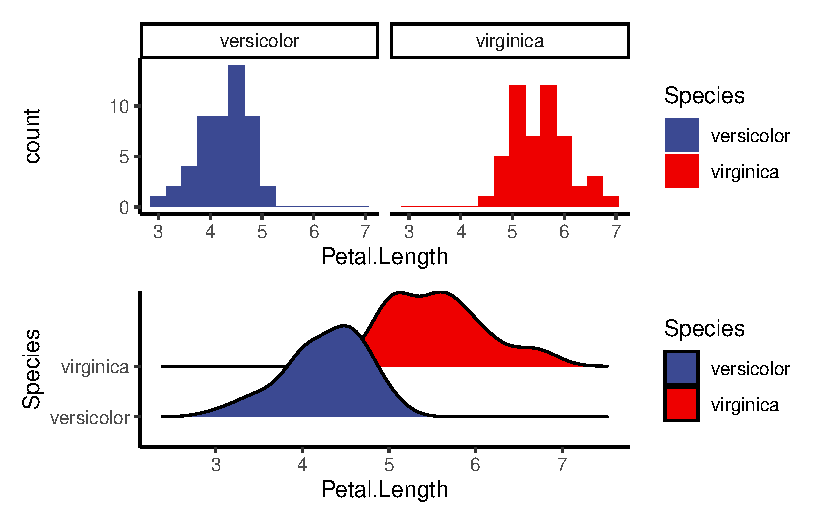
\includegraphics{t_test_files/figure-pdf/unnamed-chunk-5-1.pdf}

}

\end{figure}

\begin{Shaded}
\begin{Highlighting}[]
\NormalTok{b1}\OtherTok{\textless{}{-}}\FunctionTok{ggplot}\NormalTok{(}\AttributeTok{data=}\NormalTok{iris2, }\FunctionTok{aes}\NormalTok{(Petal.Width, }\AttributeTok{fill=}\NormalTok{Species))}\SpecialCharTok{+}
  \FunctionTok{geom\_histogram}\NormalTok{(}\AttributeTok{binwidth =} \FloatTok{0.3}\NormalTok{)}\SpecialCharTok{+} 
  \FunctionTok{facet\_wrap}\NormalTok{(}\SpecialCharTok{\textasciitilde{}}\NormalTok{Species)}\SpecialCharTok{+}
  \FunctionTok{theme\_classic}\NormalTok{()}\SpecialCharTok{+}
  \FunctionTok{scale\_fill\_aaas}\NormalTok{()}

\NormalTok{b2}\OtherTok{\textless{}{-}}\FunctionTok{ggplot}\NormalTok{(}\AttributeTok{data=}\NormalTok{iris2, }\FunctionTok{aes}\NormalTok{(}\AttributeTok{x=}\NormalTok{Petal.Width, }\AttributeTok{y=}\NormalTok{Species, }\AttributeTok{fill=}\NormalTok{Species))}\SpecialCharTok{+}
  \FunctionTok{geom\_density\_ridges}\NormalTok{()}\SpecialCharTok{+} \CommentTok{\#makes a smooth density curve instead of a histogram!}
  \FunctionTok{theme\_classic}\NormalTok{()}\SpecialCharTok{+}
  \FunctionTok{scale\_fill\_aaas}\NormalTok{()}

\NormalTok{b1}\SpecialCharTok{/}\NormalTok{b2 }\CommentTok{\#compare the visualizations (they are of the same data){-} do we see normality here?}
\end{Highlighting}
\end{Shaded}

\begin{verbatim}
Picking joint bandwidth of 0.0972
\end{verbatim}

\begin{figure}[H]

{\centering 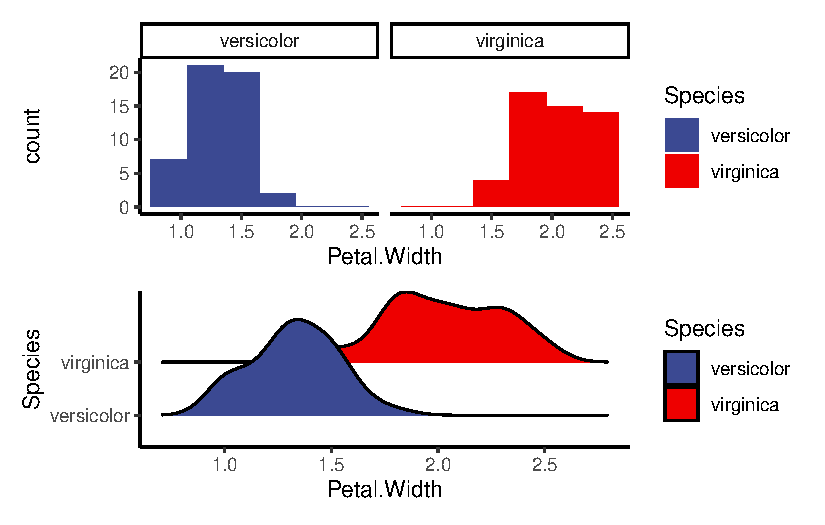
\includegraphics{t_test_files/figure-pdf/unnamed-chunk-6-1.pdf}

}

\end{figure}

\begin{Shaded}
\begin{Highlighting}[]
\NormalTok{c1}\OtherTok{\textless{}{-}}\FunctionTok{ggplot}\NormalTok{(}\AttributeTok{data=}\NormalTok{iris2, }\FunctionTok{aes}\NormalTok{(Sepal.Width, }\AttributeTok{fill=}\NormalTok{Species))}\SpecialCharTok{+}
  \FunctionTok{geom\_histogram}\NormalTok{(}\AttributeTok{binwidth =} \FloatTok{0.3}\NormalTok{)}\SpecialCharTok{+} 
  \FunctionTok{facet\_wrap}\NormalTok{(}\SpecialCharTok{\textasciitilde{}}\NormalTok{Species)}\SpecialCharTok{+}
  \FunctionTok{theme\_classic}\NormalTok{()}\SpecialCharTok{+}
  \FunctionTok{scale\_fill\_aaas}\NormalTok{()}

\NormalTok{c2}\OtherTok{\textless{}{-}}\FunctionTok{ggplot}\NormalTok{(}\AttributeTok{data=}\NormalTok{iris2, }\FunctionTok{aes}\NormalTok{(}\AttributeTok{x=}\NormalTok{Sepal.Width, }\AttributeTok{y=}\NormalTok{Species, }\AttributeTok{fill=}\NormalTok{Species))}\SpecialCharTok{+}
  \FunctionTok{geom\_density\_ridges}\NormalTok{()}\SpecialCharTok{+} \CommentTok{\#makes a smooth density curve instead of a histogram!}
  \FunctionTok{theme\_classic}\NormalTok{()}\SpecialCharTok{+}
  \FunctionTok{scale\_fill\_aaas}\NormalTok{()}

\NormalTok{c1}\SpecialCharTok{/}\NormalTok{c2 }\CommentTok{\#compare the visualizations (they are of the same data){-} do we see normality here?}
\end{Highlighting}
\end{Shaded}

\begin{verbatim}
Picking joint bandwidth of 0.122
\end{verbatim}

\begin{figure}[H]

{\centering 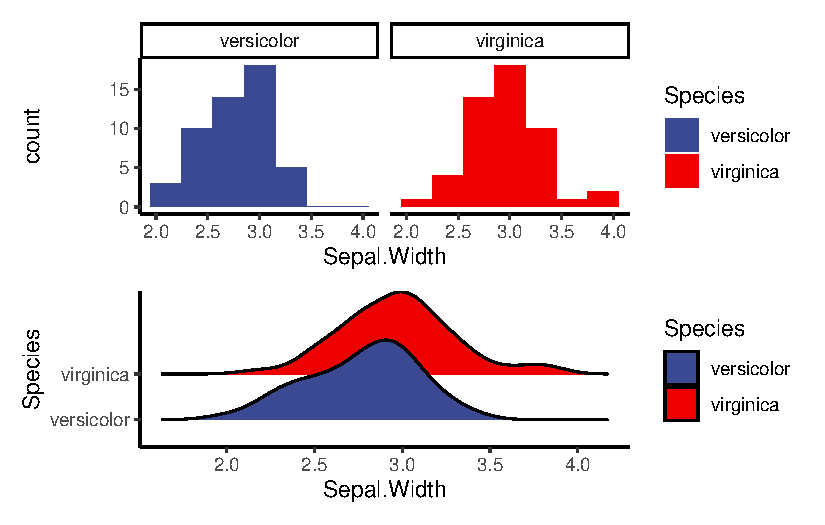
\includegraphics{t_test_files/figure-pdf/unnamed-chunk-7-1.pdf}

}

\end{figure}

\begin{Shaded}
\begin{Highlighting}[]
\NormalTok{d1}\OtherTok{\textless{}{-}}\FunctionTok{ggplot}\NormalTok{(}\AttributeTok{data=}\NormalTok{iris2, }\FunctionTok{aes}\NormalTok{(Sepal.Length, }\AttributeTok{fill=}\NormalTok{Species))}\SpecialCharTok{+}
  \FunctionTok{geom\_histogram}\NormalTok{(}\AttributeTok{binwidth =} \FloatTok{0.3}\NormalTok{)}\SpecialCharTok{+} 
  \FunctionTok{facet\_wrap}\NormalTok{(}\SpecialCharTok{\textasciitilde{}}\NormalTok{Species)}\SpecialCharTok{+}
  \FunctionTok{theme\_classic}\NormalTok{()}\SpecialCharTok{+}
  \FunctionTok{scale\_fill\_aaas}\NormalTok{()}

\NormalTok{d2}\OtherTok{\textless{}{-}}\FunctionTok{ggplot}\NormalTok{(}\AttributeTok{data=}\NormalTok{iris2, }\FunctionTok{aes}\NormalTok{(}\AttributeTok{x=}\NormalTok{Sepal.Length, }\AttributeTok{y=}\NormalTok{Species, }\AttributeTok{fill=}\NormalTok{Species))}\SpecialCharTok{+}
  \FunctionTok{geom\_density\_ridges}\NormalTok{()}\SpecialCharTok{+} \CommentTok{\#makes a smooth density curve instead of a histogram!}
  \FunctionTok{theme\_classic}\NormalTok{()}\SpecialCharTok{+}
  \FunctionTok{scale\_fill\_aaas}\NormalTok{()}

\NormalTok{d1}\SpecialCharTok{/}\NormalTok{d2 }\CommentTok{\#compare the visualizations (they are of the same data){-} do we see normality here?}
\end{Highlighting}
\end{Shaded}

\begin{verbatim}
Picking joint bandwidth of 0.21
\end{verbatim}

\begin{figure}[H]

{\centering 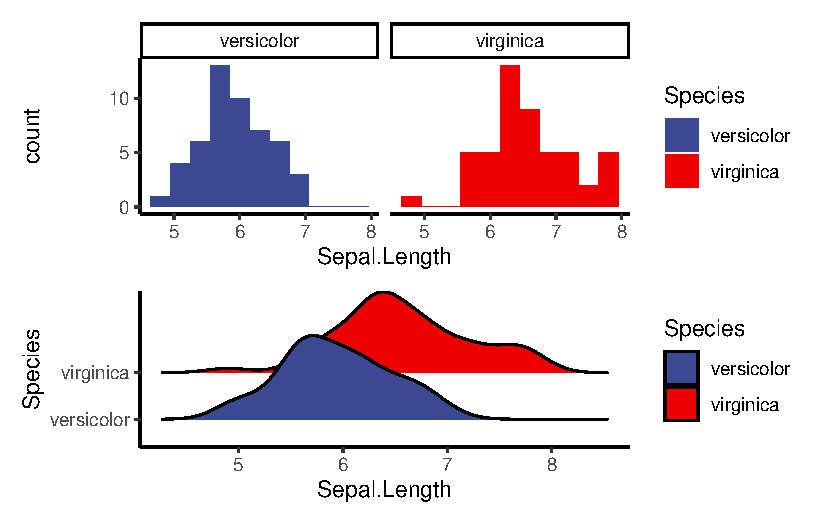
\includegraphics{t_test_files/figure-pdf/unnamed-chunk-8-1.pdf}

}

\end{figure}

\hypertarget{assumption-2.-assessing-equal-variance}{%
\subsection{\texorpdfstring{\textbf{Assumption 2.) Assessing equal
variance}}{Assumption 2.) Assessing equal variance}}\label{assumption-2.-assessing-equal-variance}}

AKA homogeneity of variance\\

\textbf{Methods 1: F-test} We will use the \textbf{F-Test} to compare
the variance of two populations. This can only be used with \emph{2}
populations and is thus only useful when we run a t-test.

H0 for an F-test is: The variances of the two groups are equal.\\
Ha: The variances are different\\
p\textless0.05 allows us to reject the null (H0) and suggests that the
variances are different\\
\strut \\
\textbf{note:} The F-test assumes our data are already normal! You
should not run it on non-normal data

\begin{Shaded}
\begin{Highlighting}[]
\CommentTok{\#we use var.test to run an F{-}test}
\NormalTok{f1}\OtherTok{\textless{}{-}} \FunctionTok{var.test}\NormalTok{(Petal.Length }\SpecialCharTok{\textasciitilde{}}\NormalTok{ Species, }\AttributeTok{data=}\NormalTok{iris2)}
\NormalTok{f1 }\CommentTok{\# p\textgreater{}0.05, so we fail to reject H0 (the variances are likely equal)}
\end{Highlighting}
\end{Shaded}

\begin{verbatim}

    F test to compare two variances

data:  Petal.Length by Species
F = 0.72497, num df = 49, denom df = 49, p-value = 0.2637
alternative hypothesis: true ratio of variances is not equal to 1
95 percent confidence interval:
 0.411402 1.277530
sample estimates:
ratio of variances 
         0.7249678 
\end{verbatim}

\begin{Shaded}
\begin{Highlighting}[]
\NormalTok{f2}\OtherTok{\textless{}{-}} \FunctionTok{var.test}\NormalTok{(Petal.Width }\SpecialCharTok{\textasciitilde{}}\NormalTok{ Species, }\AttributeTok{data=}\NormalTok{iris2)}
\NormalTok{f2 }\CommentTok{\# p\textless{}0.05, so we reject H0 (variances are likely different)}
\end{Highlighting}
\end{Shaded}

\begin{verbatim}

    F test to compare two variances

data:  Petal.Width by Species
F = 0.51842, num df = 49, denom df = 49, p-value = 0.02335
alternative hypothesis: true ratio of variances is not equal to 1
95 percent confidence interval:
 0.2941935 0.9135614
sample estimates:
ratio of variances 
         0.5184243 
\end{verbatim}

\begin{Shaded}
\begin{Highlighting}[]
\NormalTok{f3}\OtherTok{\textless{}{-}} \FunctionTok{var.test}\NormalTok{(Sepal.Length }\SpecialCharTok{\textasciitilde{}}\NormalTok{ Species, }\AttributeTok{data=}\NormalTok{iris2)}
\NormalTok{f3 }\CommentTok{\# p\textgreater{}0.05, so we fail to reject H0 (the variances are likely equal)}
\end{Highlighting}
\end{Shaded}

\begin{verbatim}

    F test to compare two variances

data:  Sepal.Length by Species
F = 0.65893, num df = 49, denom df = 49, p-value = 0.1478
alternative hypothesis: true ratio of variances is not equal to 1
95 percent confidence interval:
 0.3739257 1.1611546
sample estimates:
ratio of variances 
         0.6589276 
\end{verbatim}

\begin{Shaded}
\begin{Highlighting}[]
\NormalTok{f4}\OtherTok{\textless{}{-}} \FunctionTok{var.test}\NormalTok{(Sepal.Width }\SpecialCharTok{\textasciitilde{}}\NormalTok{ Species, }\AttributeTok{data=}\NormalTok{iris2)}
\NormalTok{f4 }\CommentTok{\# p\textgreater{}0.05, so we fail to reject H0 (the variances are likely equal)}
\end{Highlighting}
\end{Shaded}

\begin{verbatim}

    F test to compare two variances

data:  Sepal.Width by Species
F = 0.94678, num df = 49, denom df = 49, p-value = 0.849
alternative hypothesis: true ratio of variances is not equal to 1
95 percent confidence interval:
 0.5372773 1.6684117
sample estimates:
ratio of variances 
         0.9467839 
\end{verbatim}

\hfill\break
\textbf{Method 2: Levene Test}\\
A more flexible test of homogeneity of variance is the Levene Test. It
can be used to compare the variance of many populations (not just 2) and
is more flexible than the F-test, so it can be used even if the
normality assumption is violated.\\
\textbf{this is the most commonly used test for homogeneity of
variance}\\
\textbf{leveneTest() is in the car package in R!}\\

N0: Variances of all populations are equal\\
p\textless0.05 allows us to reject H0

\begin{Shaded}
\begin{Highlighting}[]
\NormalTok{l1}\OtherTok{\textless{}{-}} \FunctionTok{leveneTest}\NormalTok{(Petal.Length }\SpecialCharTok{\textasciitilde{}}\NormalTok{ Species, }\AttributeTok{data=}\NormalTok{iris2)}
\NormalTok{l1 }\CommentTok{\# p\textgreater{}0.05, so we fail to reject H0 (the variances are likely equal)}
\end{Highlighting}
\end{Shaded}

\begin{verbatim}
Levene's Test for Homogeneity of Variance (center = median)
      Df F value Pr(>F)
group  1  1.0674 0.3041
      98               
\end{verbatim}

\begin{Shaded}
\begin{Highlighting}[]
\NormalTok{l2}\OtherTok{\textless{}{-}} \FunctionTok{leveneTest}\NormalTok{(Petal.Width }\SpecialCharTok{\textasciitilde{}}\NormalTok{ Species, }\AttributeTok{data=}\NormalTok{iris2)}
\NormalTok{l2 }\CommentTok{\# p\textless{}0.05, so we reject H0 (variances are likely different)}
\end{Highlighting}
\end{Shaded}

\begin{verbatim}
Levene's Test for Homogeneity of Variance (center = median)
      Df F value  Pr(>F)  
group  1  6.5455 0.01205 *
      98                  
---
Signif. codes:  0 '***' 0.001 '**' 0.01 '*' 0.05 '.' 0.1 ' ' 1
\end{verbatim}

\begin{Shaded}
\begin{Highlighting}[]
\NormalTok{l3}\OtherTok{\textless{}{-}} \FunctionTok{leveneTest}\NormalTok{(Sepal.Length }\SpecialCharTok{\textasciitilde{}}\NormalTok{ Species, }\AttributeTok{data=}\NormalTok{iris2)}
\NormalTok{l3 }\CommentTok{\# p\textgreater{}0.05, so we fail to reject H0 (the variances are likely equal)}
\end{Highlighting}
\end{Shaded}

\begin{verbatim}
Levene's Test for Homogeneity of Variance (center = median)
      Df F value Pr(>F)
group  1  1.0245 0.3139
      98               
\end{verbatim}

\begin{Shaded}
\begin{Highlighting}[]
\NormalTok{l4}\OtherTok{\textless{}{-}} \FunctionTok{leveneTest}\NormalTok{(Sepal.Width }\SpecialCharTok{\textasciitilde{}}\NormalTok{ Species, }\AttributeTok{data=}\NormalTok{iris2)}
\NormalTok{l4 }\CommentTok{\# p\textgreater{}0.05, so we fail to reject H0 (the variances are likely equal)}
\end{Highlighting}
\end{Shaded}

\begin{verbatim}
Levene's Test for Homogeneity of Variance (center = median)
      Df F value Pr(>F)
group  1  0.0873 0.7683
      98               
\end{verbatim}

\hfill\break
\textbf{Method 3: Visualization}\\
Since p-values are more like guidelines, we also want to visualize our
data to assess homogeneity of variance. We can do that in several ways.
You might already have some ideas about this! In general, it seems smart
to display the raw data as points and as boxplots. Let's start there!

\begin{Shaded}
\begin{Highlighting}[]
\NormalTok{v1}\FloatTok{.1}\OtherTok{\textless{}{-}}\FunctionTok{ggplot}\NormalTok{(}\AttributeTok{data=}\NormalTok{iris2, }\FunctionTok{aes}\NormalTok{(}\AttributeTok{x=}\NormalTok{Species, }\AttributeTok{y=}\NormalTok{Petal.Length, }\AttributeTok{color=}\NormalTok{Species))}\SpecialCharTok{+}
  \FunctionTok{geom\_point}\NormalTok{()}\SpecialCharTok{+}
  \FunctionTok{theme\_classic}\NormalTok{()}\SpecialCharTok{+}
  \FunctionTok{scale\_color\_aaas}\NormalTok{()}

\NormalTok{v1}\FloatTok{.2}\OtherTok{\textless{}{-}}\FunctionTok{ggplot}\NormalTok{(}\AttributeTok{data=}\NormalTok{iris2, }\FunctionTok{aes}\NormalTok{(}\AttributeTok{x=}\NormalTok{Species, }\AttributeTok{y=}\NormalTok{Petal.Length, }\AttributeTok{color=}\NormalTok{Species))}\SpecialCharTok{+}
  \FunctionTok{geom\_boxplot}\NormalTok{()}\SpecialCharTok{+}
  \FunctionTok{theme\_classic}\NormalTok{()}\SpecialCharTok{+}
  \FunctionTok{scale\_color\_aaas}\NormalTok{()}

\NormalTok{v1}\FloatTok{.1}\SpecialCharTok{+}\NormalTok{v1}\FloatTok{.2}
\end{Highlighting}
\end{Shaded}

\begin{figure}[H]

{\centering 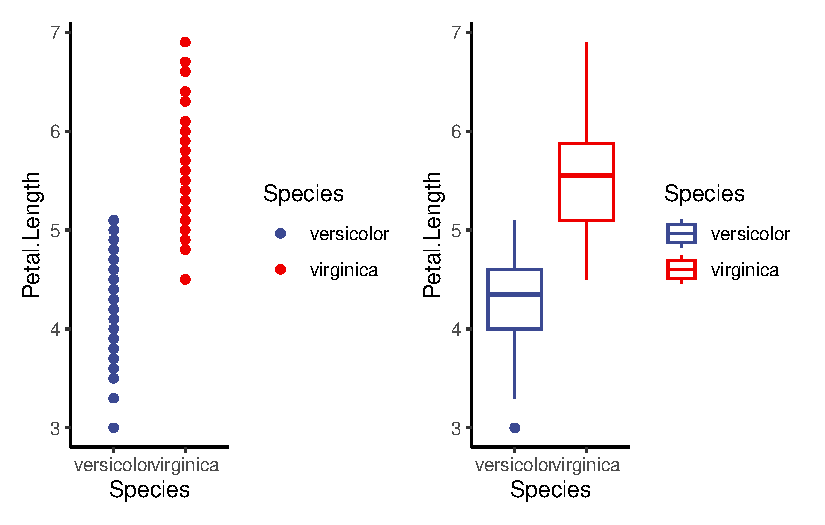
\includegraphics{t_test_files/figure-pdf/unnamed-chunk-11-1.pdf}

}

\end{figure}

\begin{Shaded}
\begin{Highlighting}[]
\NormalTok{v2}\FloatTok{.1}\OtherTok{\textless{}{-}}\FunctionTok{ggplot}\NormalTok{(}\AttributeTok{data=}\NormalTok{iris2, }\FunctionTok{aes}\NormalTok{(}\AttributeTok{x=}\NormalTok{Species, }\AttributeTok{y=}\NormalTok{Petal.Width, }\AttributeTok{color=}\NormalTok{Species))}\SpecialCharTok{+}
  \FunctionTok{geom\_point}\NormalTok{()}\SpecialCharTok{+}
  \FunctionTok{theme\_classic}\NormalTok{()}\SpecialCharTok{+}
  \FunctionTok{scale\_color\_aaas}\NormalTok{()}

\NormalTok{v2}\FloatTok{.2}\OtherTok{\textless{}{-}}\FunctionTok{ggplot}\NormalTok{(}\AttributeTok{data=}\NormalTok{iris2, }\FunctionTok{aes}\NormalTok{(}\AttributeTok{x=}\NormalTok{Species, }\AttributeTok{y=}\NormalTok{Petal.Width, }\AttributeTok{color=}\NormalTok{Species))}\SpecialCharTok{+}
  \FunctionTok{geom\_boxplot}\NormalTok{()}\SpecialCharTok{+}
  \FunctionTok{theme\_classic}\NormalTok{()}\SpecialCharTok{+}
  \FunctionTok{scale\_color\_aaas}\NormalTok{()}

\NormalTok{v2}\FloatTok{.1}\SpecialCharTok{+}\NormalTok{v2}\FloatTok{.2}
\end{Highlighting}
\end{Shaded}

\begin{figure}[H]

{\centering 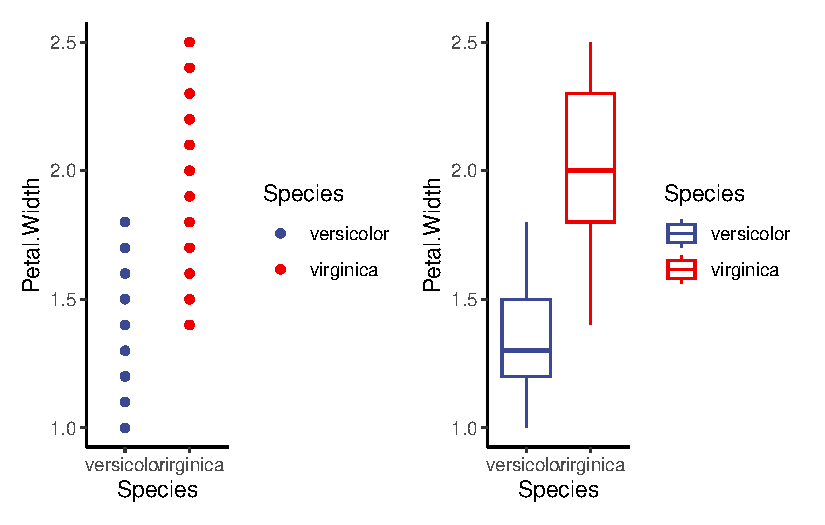
\includegraphics{t_test_files/figure-pdf/unnamed-chunk-12-1.pdf}

}

\end{figure}

\begin{Shaded}
\begin{Highlighting}[]
\NormalTok{v3}\FloatTok{.1}\OtherTok{\textless{}{-}}\FunctionTok{ggplot}\NormalTok{(}\AttributeTok{data=}\NormalTok{iris2, }\FunctionTok{aes}\NormalTok{(}\AttributeTok{x=}\NormalTok{Species, }\AttributeTok{y=}\NormalTok{Sepal.Width, }\AttributeTok{color=}\NormalTok{Species))}\SpecialCharTok{+}
  \FunctionTok{geom\_point}\NormalTok{()}\SpecialCharTok{+}
  \FunctionTok{theme\_classic}\NormalTok{()}\SpecialCharTok{+}
  \FunctionTok{scale\_color\_aaas}\NormalTok{()}

\NormalTok{v3}\FloatTok{.2}\OtherTok{\textless{}{-}}\FunctionTok{ggplot}\NormalTok{(}\AttributeTok{data=}\NormalTok{iris2, }\FunctionTok{aes}\NormalTok{(}\AttributeTok{x=}\NormalTok{Species, }\AttributeTok{y=}\NormalTok{Sepal.Width, }\AttributeTok{color=}\NormalTok{Species))}\SpecialCharTok{+}
  \FunctionTok{geom\_boxplot}\NormalTok{()}\SpecialCharTok{+}
  \FunctionTok{theme\_classic}\NormalTok{()}\SpecialCharTok{+}
  \FunctionTok{scale\_color\_aaas}\NormalTok{()}

\NormalTok{v3}\FloatTok{.1}\SpecialCharTok{+}\NormalTok{v3}\FloatTok{.2}
\end{Highlighting}
\end{Shaded}

\begin{figure}[H]

{\centering 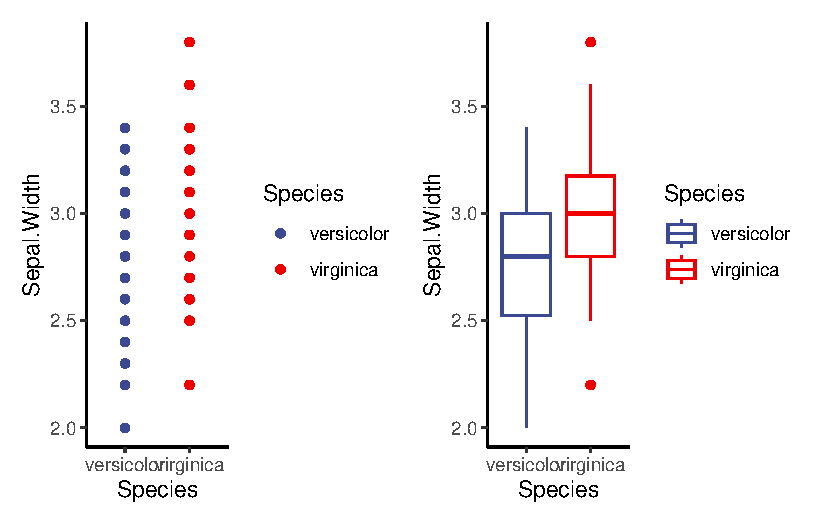
\includegraphics{t_test_files/figure-pdf/unnamed-chunk-13-1.pdf}

}

\end{figure}

\begin{Shaded}
\begin{Highlighting}[]
\NormalTok{v4}\FloatTok{.1}\OtherTok{\textless{}{-}}\FunctionTok{ggplot}\NormalTok{(}\AttributeTok{data=}\NormalTok{iris2, }\FunctionTok{aes}\NormalTok{(}\AttributeTok{x=}\NormalTok{Species, }\AttributeTok{y=}\NormalTok{Sepal.Length, }\AttributeTok{color=}\NormalTok{Species))}\SpecialCharTok{+}
  \FunctionTok{geom\_point}\NormalTok{()}\SpecialCharTok{+}
  \FunctionTok{theme\_classic}\NormalTok{()}\SpecialCharTok{+}
  \FunctionTok{scale\_color\_aaas}\NormalTok{()}

\NormalTok{v4}\FloatTok{.2}\OtherTok{\textless{}{-}}\FunctionTok{ggplot}\NormalTok{(}\AttributeTok{data=}\NormalTok{iris2, }\FunctionTok{aes}\NormalTok{(}\AttributeTok{x=}\NormalTok{Species, }\AttributeTok{y=}\NormalTok{Sepal.Length, }\AttributeTok{color=}\NormalTok{Species))}\SpecialCharTok{+}
  \FunctionTok{geom\_boxplot}\NormalTok{()}\SpecialCharTok{+}
  \FunctionTok{theme\_classic}\NormalTok{()}\SpecialCharTok{+}
  \FunctionTok{scale\_color\_aaas}\NormalTok{()}

\NormalTok{v4}\FloatTok{.1}\SpecialCharTok{+}\NormalTok{v4}\FloatTok{.2}
\end{Highlighting}
\end{Shaded}

\begin{figure}[H]

{\centering 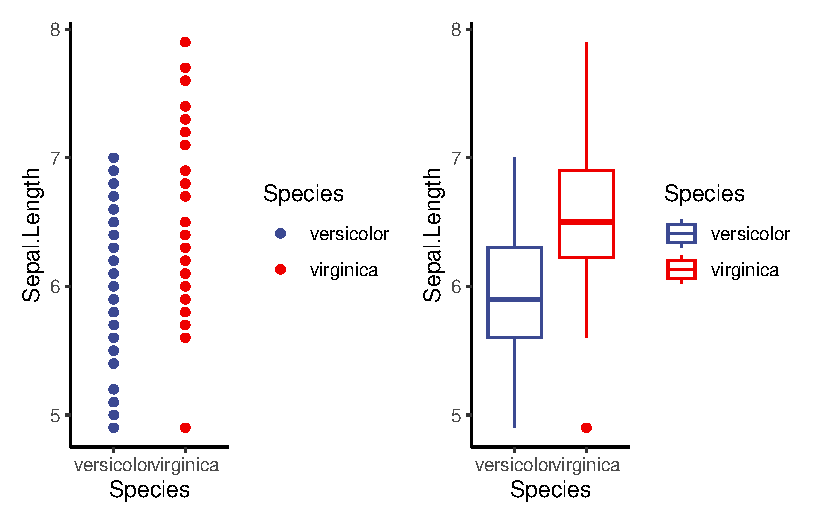
\includegraphics{t_test_files/figure-pdf/unnamed-chunk-14-1.pdf}

}

\end{figure}

\hypertarget{when-can-we-ignore-assumptions}{%
\subsection{\texorpdfstring{\textbf{When can we ignore
assumptions?}}{When can we ignore assumptions?}}\label{when-can-we-ignore-assumptions}}

We can if our sample sizes are large. If n is small, we should not
ignore this assumption. There are alternatives to dealing with normality
that we can discuss in the ANOVA section (such as transforming the data)

\href{https://thestatsgeek.com/2013/09/28/the-t-test-and-robustness-to-non-normality/}{For
more info on that}

We can also ignore the equal variance requirement if we use the Welch
t-test (default in R)\\

\hypertarget{a-basic-t-test-in-r}{%
\subsection{\texorpdfstring{\textbf{A basic T-test in
R}}{A basic T-test in R}}\label{a-basic-t-test-in-r}}

Finally, let's do some T-tests!\\

H0: No difference between the means of the 2 populations p\textless0.05
allows us to reject this H0 (indicating a likely difference)

\textbf{Step 1:} Calculate means and error and plot!

\begin{Shaded}
\begin{Highlighting}[]
\NormalTok{meaniris}\OtherTok{\textless{}{-}}\NormalTok{iris2 }\SpecialCharTok{\%\textgreater{}\%}
  \FunctionTok{group\_by}\NormalTok{(Species) }\SpecialCharTok{\%\textgreater{}\%}
\NormalTok{  dplyr}\SpecialCharTok{::}\FunctionTok{summarise}\NormalTok{(}\AttributeTok{meanpl=}\FunctionTok{mean}\NormalTok{(Petal.Length), }\AttributeTok{sdpl=}\FunctionTok{sd}\NormalTok{(Petal.Length), }\AttributeTok{n=}\FunctionTok{n}\NormalTok{(), }\AttributeTok{sepl=}\NormalTok{sdpl}\SpecialCharTok{/}\FunctionTok{sqrt}\NormalTok{(n), }\AttributeTok{meanpw=}\FunctionTok{mean}\NormalTok{(Petal.Width), }\AttributeTok{sdpw=}\FunctionTok{sd}\NormalTok{(Petal.Width), }\AttributeTok{n=}\FunctionTok{n}\NormalTok{(), }\AttributeTok{sepw=}\NormalTok{sdpw}\SpecialCharTok{/}\FunctionTok{sqrt}\NormalTok{(n), }\AttributeTok{meansl=}\FunctionTok{mean}\NormalTok{(Sepal.Length), }\AttributeTok{sdsl=}\FunctionTok{sd}\NormalTok{(Sepal.Length), }\AttributeTok{n=}\FunctionTok{n}\NormalTok{(), }\AttributeTok{sesl=}\NormalTok{sdpl}\SpecialCharTok{/}\FunctionTok{sqrt}\NormalTok{(n), }\AttributeTok{meansw=}\FunctionTok{mean}\NormalTok{(Sepal.Width), }\AttributeTok{sdsw=}\FunctionTok{sd}\NormalTok{(Sepal.Width), }\AttributeTok{n=}\FunctionTok{n}\NormalTok{(), }\AttributeTok{sesw=}\NormalTok{sdsw}\SpecialCharTok{/}\FunctionTok{sqrt}\NormalTok{(n))}

\NormalTok{meaniris}
\end{Highlighting}
\end{Shaded}

\begin{verbatim}
# A tibble: 2 x 14
  Species    meanpl  sdpl     n   sepl meanpw  sdpw   sepw meansl  sdsl   sesl
  <fct>       <dbl> <dbl> <int>  <dbl>  <dbl> <dbl>  <dbl>  <dbl> <dbl>  <dbl>
1 versicolor   4.26 0.470    50 0.0665   1.33 0.198 0.0280   5.94 0.516 0.0665
2 virginica    5.55 0.552    50 0.0780   2.03 0.275 0.0388   6.59 0.636 0.0780
# i 3 more variables: meansw <dbl>, sdsw <dbl>, sesw <dbl>
\end{verbatim}

\hfill\break

\begin{Shaded}
\begin{Highlighting}[]
\NormalTok{p1}\OtherTok{\textless{}{-}}\FunctionTok{ggplot}\NormalTok{(meaniris, }\FunctionTok{aes}\NormalTok{(}\AttributeTok{x=}\NormalTok{Species, }\AttributeTok{y=}\NormalTok{meanpl, }\AttributeTok{color=}\NormalTok{Species))}\SpecialCharTok{+}
  \FunctionTok{geom\_point}\NormalTok{()}\SpecialCharTok{+}
  \FunctionTok{geom\_errorbar}\NormalTok{(}\FunctionTok{aes}\NormalTok{(}\AttributeTok{x=}\NormalTok{Species, }\AttributeTok{ymin=}\NormalTok{meanpl}\SpecialCharTok{{-}}\NormalTok{sepl, }\AttributeTok{ymax=}\NormalTok{meanpl}\SpecialCharTok{+}\NormalTok{sepl), }\AttributeTok{width=}\FloatTok{0.2}\NormalTok{)}\SpecialCharTok{+}
  \FunctionTok{scale\_color\_aaas}\NormalTok{()}\SpecialCharTok{+}
  \FunctionTok{theme\_classic}\NormalTok{()}\SpecialCharTok{+}
  \FunctionTok{labs}\NormalTok{(}\AttributeTok{title=}\StringTok{\textquotesingle{}Petal Length\textquotesingle{}}\NormalTok{)}

\NormalTok{p2}\OtherTok{\textless{}{-}}\FunctionTok{ggplot}\NormalTok{(meaniris, }\FunctionTok{aes}\NormalTok{(}\AttributeTok{x=}\NormalTok{Species, }\AttributeTok{y=}\NormalTok{meanpw, }\AttributeTok{color=}\NormalTok{Species))}\SpecialCharTok{+}
  \FunctionTok{geom\_point}\NormalTok{()}\SpecialCharTok{+}
  \FunctionTok{geom\_errorbar}\NormalTok{(}\FunctionTok{aes}\NormalTok{(}\AttributeTok{x=}\NormalTok{Species, }\AttributeTok{ymin=}\NormalTok{meanpw}\SpecialCharTok{{-}}\NormalTok{sepw, }\AttributeTok{ymax=}\NormalTok{meanpw}\SpecialCharTok{+}\NormalTok{sepw), }\AttributeTok{width=}\FloatTok{0.2}\NormalTok{)}\SpecialCharTok{+}
  \FunctionTok{scale\_color\_aaas}\NormalTok{()}\SpecialCharTok{+}
  \FunctionTok{theme\_classic}\NormalTok{()}\SpecialCharTok{+}
  \FunctionTok{labs}\NormalTok{(}\AttributeTok{title=}\StringTok{\textquotesingle{}Petal Width\textquotesingle{}}\NormalTok{)}

\NormalTok{p3}\OtherTok{\textless{}{-}}\FunctionTok{ggplot}\NormalTok{(meaniris, }\FunctionTok{aes}\NormalTok{(}\AttributeTok{x=}\NormalTok{Species, }\AttributeTok{y=}\NormalTok{meansl, }\AttributeTok{color=}\NormalTok{Species))}\SpecialCharTok{+}
  \FunctionTok{geom\_point}\NormalTok{()}\SpecialCharTok{+}
  \FunctionTok{geom\_errorbar}\NormalTok{(}\FunctionTok{aes}\NormalTok{(}\AttributeTok{x=}\NormalTok{Species, }\AttributeTok{ymin=}\NormalTok{meansl}\SpecialCharTok{{-}}\NormalTok{sesl, }\AttributeTok{ymax=}\NormalTok{meansl}\SpecialCharTok{+}\NormalTok{sesl), }\AttributeTok{width=}\FloatTok{0.2}\NormalTok{)}\SpecialCharTok{+}
  \FunctionTok{scale\_color\_aaas}\NormalTok{()}\SpecialCharTok{+}
  \FunctionTok{theme\_classic}\NormalTok{()}\SpecialCharTok{+}
  \FunctionTok{labs}\NormalTok{(}\AttributeTok{title=}\StringTok{\textquotesingle{}Sepal Length\textquotesingle{}}\NormalTok{)}

\NormalTok{p4}\OtherTok{\textless{}{-}}\FunctionTok{ggplot}\NormalTok{(meaniris, }\FunctionTok{aes}\NormalTok{(}\AttributeTok{x=}\NormalTok{Species, }\AttributeTok{y=}\NormalTok{meansw, }\AttributeTok{color=}\NormalTok{Species))}\SpecialCharTok{+}
  \FunctionTok{geom\_point}\NormalTok{()}\SpecialCharTok{+}
  \FunctionTok{geom\_errorbar}\NormalTok{(}\FunctionTok{aes}\NormalTok{(}\AttributeTok{x=}\NormalTok{Species, }\AttributeTok{ymin=}\NormalTok{meansw}\SpecialCharTok{{-}}\NormalTok{sesw, }\AttributeTok{ymax=}\NormalTok{meansw}\SpecialCharTok{+}\NormalTok{sesw), }\AttributeTok{width=}\FloatTok{0.2}\NormalTok{)}\SpecialCharTok{+}
  \FunctionTok{scale\_color\_aaas}\NormalTok{()}\SpecialCharTok{+}
  \FunctionTok{theme\_classic}\NormalTok{()}\SpecialCharTok{+}
  \FunctionTok{labs}\NormalTok{(}\AttributeTok{title=}\StringTok{\textquotesingle{}Sepal Width\textquotesingle{}}\NormalTok{)}

\NormalTok{(p1}\SpecialCharTok{+}\NormalTok{p2)}\SpecialCharTok{/}\NormalTok{(p3}\SpecialCharTok{+}\NormalTok{p4)}
\end{Highlighting}
\end{Shaded}

\begin{figure}[H]

{\centering 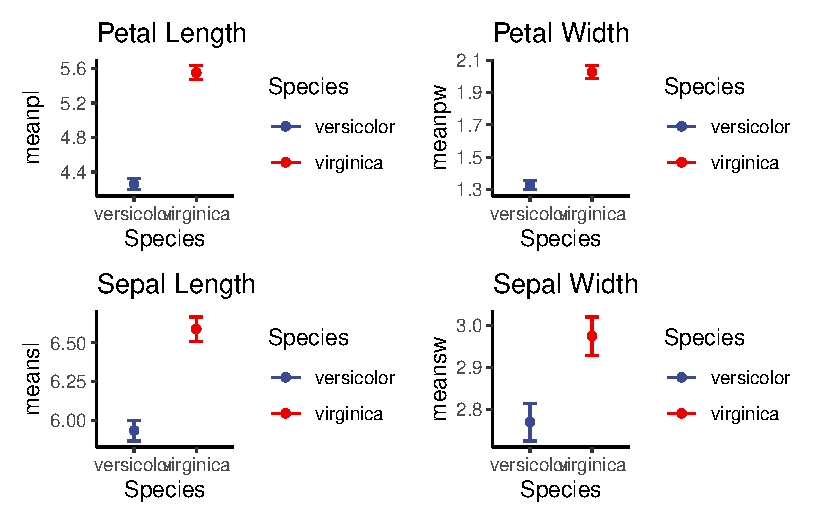
\includegraphics{t_test_files/figure-pdf/unnamed-chunk-16-1.pdf}

}

\end{figure}

\textbf{Does Petal Length differ by species?}

\begin{Shaded}
\begin{Highlighting}[]
\NormalTok{t1}\OtherTok{\textless{}{-}}\FunctionTok{t.test}\NormalTok{(}\AttributeTok{data=}\NormalTok{iris2, Petal.Length}\SpecialCharTok{\textasciitilde{}}\NormalTok{Species, }\AttributeTok{alternative=}\StringTok{\textquotesingle{}two.sided\textquotesingle{}}\NormalTok{, }\AttributeTok{var.equal=}\ConstantTok{FALSE}\NormalTok{) }\CommentTok{\#two.sided and var.equal= FALSE are default, so we don\textquotesingle{}t have to list them. BUt, we can also change them (as I will show later)}

\NormalTok{t1 }\CommentTok{\#p\textless{}0.05 suggests that there is a significant difference in petal length between species}
\end{Highlighting}
\end{Shaded}

\begin{verbatim}

    Welch Two Sample t-test

data:  Petal.Length by Species
t = -12.604, df = 95.57, p-value < 2.2e-16
alternative hypothesis: true difference in means between group versicolor and group virginica is not equal to 0
95 percent confidence interval:
 -1.49549 -1.08851
sample estimates:
mean in group versicolor  mean in group virginica 
                   4.260                    5.552 
\end{verbatim}

\hfill\break
Our p\textless0.05 suggests that there is a significant effect of
species on petal length (petal length differs by species). BUT, do we
get a clear explanation of which group is higher or lower? Look at the
Welch T-test output and you can see the means! You can also use the
graph we made to visualize this!

\textbf{Does Petal Width differ by species?}

\begin{Shaded}
\begin{Highlighting}[]
\NormalTok{t2}\OtherTok{\textless{}{-}}\FunctionTok{t.test}\NormalTok{(}\AttributeTok{data=}\NormalTok{iris2, Petal.Width}\SpecialCharTok{\textasciitilde{}}\NormalTok{Species, }\AttributeTok{alternative=}\StringTok{\textquotesingle{}two.sided\textquotesingle{}}\NormalTok{, }\AttributeTok{var.equal=}\ConstantTok{FALSE}\NormalTok{) }\CommentTok{\#two.sided and var.equal= FALSE are default, so we don\textquotesingle{}t have to list them. BUt, we can also change them (as I will show later)}

\NormalTok{t2}
\end{Highlighting}
\end{Shaded}

\begin{verbatim}

    Welch Two Sample t-test

data:  Petal.Width by Species
t = -14.625, df = 89.043, p-value < 2.2e-16
alternative hypothesis: true difference in means between group versicolor and group virginica is not equal to 0
95 percent confidence interval:
 -0.7951002 -0.6048998
sample estimates:
mean in group versicolor  mean in group virginica 
                   1.326                    2.026 
\end{verbatim}

\hfill\break
\textbf{Does Sepal Width differ between species?}

\begin{Shaded}
\begin{Highlighting}[]
\NormalTok{t3}\OtherTok{\textless{}{-}}\FunctionTok{t.test}\NormalTok{(}\AttributeTok{data=}\NormalTok{iris2, Sepal.Width}\SpecialCharTok{\textasciitilde{}}\NormalTok{Species, }\AttributeTok{alternative=}\StringTok{\textquotesingle{}two.sided\textquotesingle{}}\NormalTok{, }\AttributeTok{var.equal=}\ConstantTok{FALSE}\NormalTok{) }\CommentTok{\#two.sided and var.equal= FALSE are default, so we don\textquotesingle{}t have to list them. BUt, we can also change them (as I will show later)}

\NormalTok{t3}
\end{Highlighting}
\end{Shaded}

\begin{verbatim}

    Welch Two Sample t-test

data:  Sepal.Width by Species
t = -3.2058, df = 97.927, p-value = 0.001819
alternative hypothesis: true difference in means between group versicolor and group virginica is not equal to 0
95 percent confidence interval:
 -0.33028364 -0.07771636
sample estimates:
mean in group versicolor  mean in group virginica 
                   2.770                    2.974 
\end{verbatim}

\hfill\break
\textbf{Does Sepal Length differ between species?}

\begin{Shaded}
\begin{Highlighting}[]
\NormalTok{t4}\OtherTok{\textless{}{-}}\FunctionTok{t.test}\NormalTok{(}\AttributeTok{data=}\NormalTok{iris2, Sepal.Length}\SpecialCharTok{\textasciitilde{}}\NormalTok{Species, }\AttributeTok{alternative=}\StringTok{\textquotesingle{}two.sided\textquotesingle{}}\NormalTok{, }\AttributeTok{var.equal=}\ConstantTok{FALSE}\NormalTok{) }\CommentTok{\#two.sided and var.equal= FALSE are default, so we don\textquotesingle{}t have to list them. BUt, we can also change them (as I will show later)}

\NormalTok{t4}
\end{Highlighting}
\end{Shaded}

\begin{verbatim}

    Welch Two Sample t-test

data:  Sepal.Length by Species
t = -5.6292, df = 94.025, p-value = 1.866e-07
alternative hypothesis: true difference in means between group versicolor and group virginica is not equal to 0
95 percent confidence interval:
 -0.8819731 -0.4220269
sample estimates:
mean in group versicolor  mean in group virginica 
                   5.936                    6.588 
\end{verbatim}

SO, when is a t-test actually useful and when isn't it? We use a T-test
\textbf{ONLY} when we want to compare two means / two populations. If we
have more than 2 groups, a T-test is not appropriate! Instead, we need
to use an analysis of variance (ANOVA) or possibly something more
complex!



\end{document}
